% Soubory musí být v kódování, které je nastaveno v příkazu \usepackage[...]{inputenc}

\documentclass[%        Základní nastavení
  %draft,    				  % Testovací překlad
  12pt,       				% Velikost základního písma je 12 bodů
	t,                  % obsah slajdů bude vždy začínat od shora (nebude vertikálně centrovaný)
	aspectratio=1610,   % poměr stran bude 16:10 (všechny projektory v učebnách na Technické 12 Brno),
	                    % další volby jsou 43, 149, 169, 54, 32.
	unicode,						% Záložky a informace budou v kódování unicode
]{beamer}				    	% Dokument třídy 'zpráva', vhodná pro sazbu závěrečných prací s kapitolami
%\usepackage{etex}

\usepackage[utf8]		  % Kódování zdrojových souborů je v UTF-8
	{inputenc}					% Balíček pro nastavení kódování zdrojových souborů
	
\usepackage{graphicx} % Balíček 'graphicx' pro vkládání obrázků
											% Nutné pro vložení logotypů školy a fakulty

\usepackage[          % Balíček 'acronym' pro sazby zkratek a symbolů
	nohyperlinks				% Nebudou tvořeny hypertextové odkazy do seznamu zkratek
]{acronym}						
											% Nutné pro použití prostředí 'acronym' balíčku 'thesis'

%% Balíček hyperref je volán třídou beamer automaticky, proto není třeba následujícího kódu:
%\usepackage[
%	breaklinks=true,		% Hypertextové odkazy mohou obsahovat zalomení řádku
%	hypertexnames=false % Názvy hypertextových odkazů budou tvořeny
%											% nezávisle na názvech TeXu
%]{hyperref}						% Balíček 'hyperref' pro sazbu hypertextových odkazů
%											% Nutné pro použití příkazu 'nastavenipdf' balíčku 'thesis'

\usepackage{cmap} 		% Balíček cmap zajišťuje, že PDF vytvořené `pdflatexem' je
											% plně "prohledávatelné" a "kopírovatelné"

%\usepackage{upgreek}	% Balíček pro sazbu stojatých řeckých písmem
											%% např. stojaté pí: \uppi
											%% např. stojaté mí: \upmu (použitelné třeba v mikrometrech)
											%% pozor, grafická nekompatibilita s fonty typu Computer Modern!

%\usepackage{amsmath} %balíček pro sabu náročnější matematiky

\usepackage{booktabs} % Balíček, který umožňuje v tabulce používat
                      % příkazy \toprule, \midrule, \bottomrule


%%%%%%%%%%%%%%%%%%%%%%%%%%%%%%%%%%%%%%%%%%%%%%%%%%%%%%%%%%%%%%%%%
%%%%%%      Definice informací o dokumentu             %%%%%%%%%%
%%%%%%%%%%%%%%%%%%%%%%%%%%%%%%%%%%%%%%%%%%%%%%%%%%%%%%%%%%%%%%%%%

\input{nastaveni}      % v tomto souboru doplňte údaje o sobě, o názvu práce...
                       % (tento soubor je sdílený s textem práce)

%%%%%%%%%%%%%%%%%%%%%%%%%%%%%%%%%%%%%%%%%%%%%%%%%%%%%%%%%%%%%%%%%%%%%%%%

%%%%%%%%%%%%%%%%%%%%%%%%%%%%%%%%%%%%%%%%%%%%%%%%%%%%%%%%%%%%%%%%%%%%%%%%
%%%%%%     Nastavení polí ve Vlastnostech dokumentu PDF      %%%%%%%%%%%
%%%%%%%%%%%%%%%%%%%%%%%%%%%%%%%%%%%%%%%%%%%%%%%%%%%%%%%%%%%%%%%%%%%%%%%%
%% Při vloženém balíčku 'hyperref' lze použít příkaz '\pdfsettings'
\pdfsettings
%  Nastavení polí je možné provést také ručně příkazem:
%\hypersetup{
%  pdftitle={Název studentské práce},    	% Pole 'Document Title'
%  pdfauthor={Autor studenstké práce},   	% Pole 'Author'
%  pdfsubject={Typ práce}, 						  	% Pole 'Subject'
%  pdfkeywords={Klíčová slova}           	% Pole 'Keywords'
%}
\hypersetup{pdfpagemode=FullScreen}       % otevření rovnou v režimu celé obrazovky
%%%%%%%%%%%%%%%%%%%%%%%%%%%%%%%%%%%%%%%%%%%%%%%%%%%%%%%%%%%%%%%%%%%%%%%

\usetheme{VUT} 				% barvy a rozložení prezentace odpovídající VUT FEKT
% alternativně lze použít jiná berevná témata, ale bez záruky. Například: 
%\usetheme{Darmstadt} \usecolortheme{default2}
\logoheader					% vytvoření zkráceného loga VUT FEKT v hlavičce slajdu, nechte odkomentované



\begin{document}

% v případě zakomentování následujícího se zobrazí v pravém dolním rohu slajdů klikatelné navigační symboly 
\disablenavigationsymbols

% titulní snímek, vysazen bez horních, dolních a postranních lišt (volba plain),
% není tak vysazen ani nadpis snímku
\maketitle

%%%%%%%%%%%%%%%%%%%%%%%%%%%%%%%%%%%%%%%%%%%%%%%%%%%%%%%%%%%%%%%%%%%%%%%

\begin{frame} 
	% nadpis snímku
	\frametitle{Cíle práce}
	\begin{figure}[ht!]
		\centering
		\begin{minipage}{0.3\textwidth}
			\vspace*{-3cm}
			\begin{itemize}
				\item ICT tester
				\item Fixture
				\item Měření odporu
				\item Škálovatelnost
				\item Rychlost
			\end{itemize}
		\end{minipage}
		\begin{minipage}{0.65\textwidth}
		\includegraphics[height = 0.8\textheight]{obrazky/ICT_tester.png}
		\end{minipage}
	\end{figure}
\end{frame}

\begin{frame} 
	% nadpis snímku
	\frametitle{PASS/FAIL VS měření přesného odporu}
	\vspace*{1.5cm}
	\begin{table}[ht!]
		\resizebox{\textwidth}{!}{%
		\begin{tabular}{|lccccc|}
		\hline
		\multicolumn{6}{|c|}{\textbf{Požadované charekteristiky měřícího obvodu}}                                                                                                                                                                                                                                                                                  \\ \hline
		\multicolumn{1}{|l|}{\textbf{TEST MODE}}                & \multicolumn{1}{c|}{\textbf{Počet pinů}} & \multicolumn{1}{c|}{\textbf{Rozsah $[\Omega]$}}  & \multicolumn{1}{c|}{\textbf{Přesnost $[\pm \Omega]$}} & \multicolumn{1}{c|}{\textbf{čas $[\mu s/pin]$}} & \textbf{Celkový čas $[ms]$} \\ \hline
		\multicolumn{1}{|l|}{\textbf{PASS/FAIL}}                & \multicolumn{1}{c|}{4000}                & \multicolumn{1}{c|}{1-101}                      & \multicolumn{1}{c|}{3}                                & \multicolumn{1}{c|}{2,5}                        & 10                          \\ \hline
		\multicolumn{1}{|l|}{\textbf{PASS/FAIL}}                & \multicolumn{1}{c|}{4000}                & \multicolumn{1}{c|}{101-1000}                      & \multicolumn{1}{c|}{rel. chyba 5\%}                                & \multicolumn{1}{c|}{2,5}                        & 10                          \\ \hline
		\multicolumn{1}{|l|}{\textbf{Měření   "pravé"\ hodnoty}} & \multicolumn{1}{c|}{4000}                & \multicolumn{1}{c|}{1-101}                      & \multicolumn{1}{c|}{3}                                & \multicolumn{1}{c|}{Nedefinován}                & Nedefinován                 \\ \hline
		\multicolumn{1}{|l|}{\textbf{Měření   "pravé"\ hodnoty}} & \multicolumn{1}{c|}{4000}                & \multicolumn{1}{c|}{101-1000}                      & \multicolumn{1}{c|}{rel. chyba 5\%}                                & \multicolumn{1}{c|}{Nedefinován}                & Nedefinován                 \\ \hline
		\end{tabular}%
		}
		\caption{Požadované měřící charakteristiky}
		\label{tab:Požadované měřící charakteristiky}
	\end{table}
\end{frame}

\begin{frame} 
	% nadpis snímku
	\frametitle{Koncepce měření 1/3}
	\vspace*{0.5cm}
	\begin{figure}[ht!]
		\centering
		%\includegraphics[width = \textwidth]{obrazky/system_connection.png}
		\includegraphics[width = \textwidth]{obrazky/2_and_4_pins_connection.png}
	\end{figure}
\end{frame}

\begin{frame} 
	% nadpis snímku
	\frametitle{Koncepce měření 2/3}
	\vspace*{0.5cm}
	\begin{figure}[ht!]
		\centering
		%\includegraphics[width = \textwidth]{obrazky/system_connection.png}
		\includegraphics[width = \textwidth]{obrazky/R_meas_obhj.png}
	\end{figure}
\end{frame}

\begin{frame} 
	% nadpis snímku
	\frametitle{Koncepce měření 3/3}
	\vspace*{0.5cm}
	\begin{figure}[ht!]
		\centering
		%\includegraphics[width = \textwidth]{obrazky/system_connection.png}
		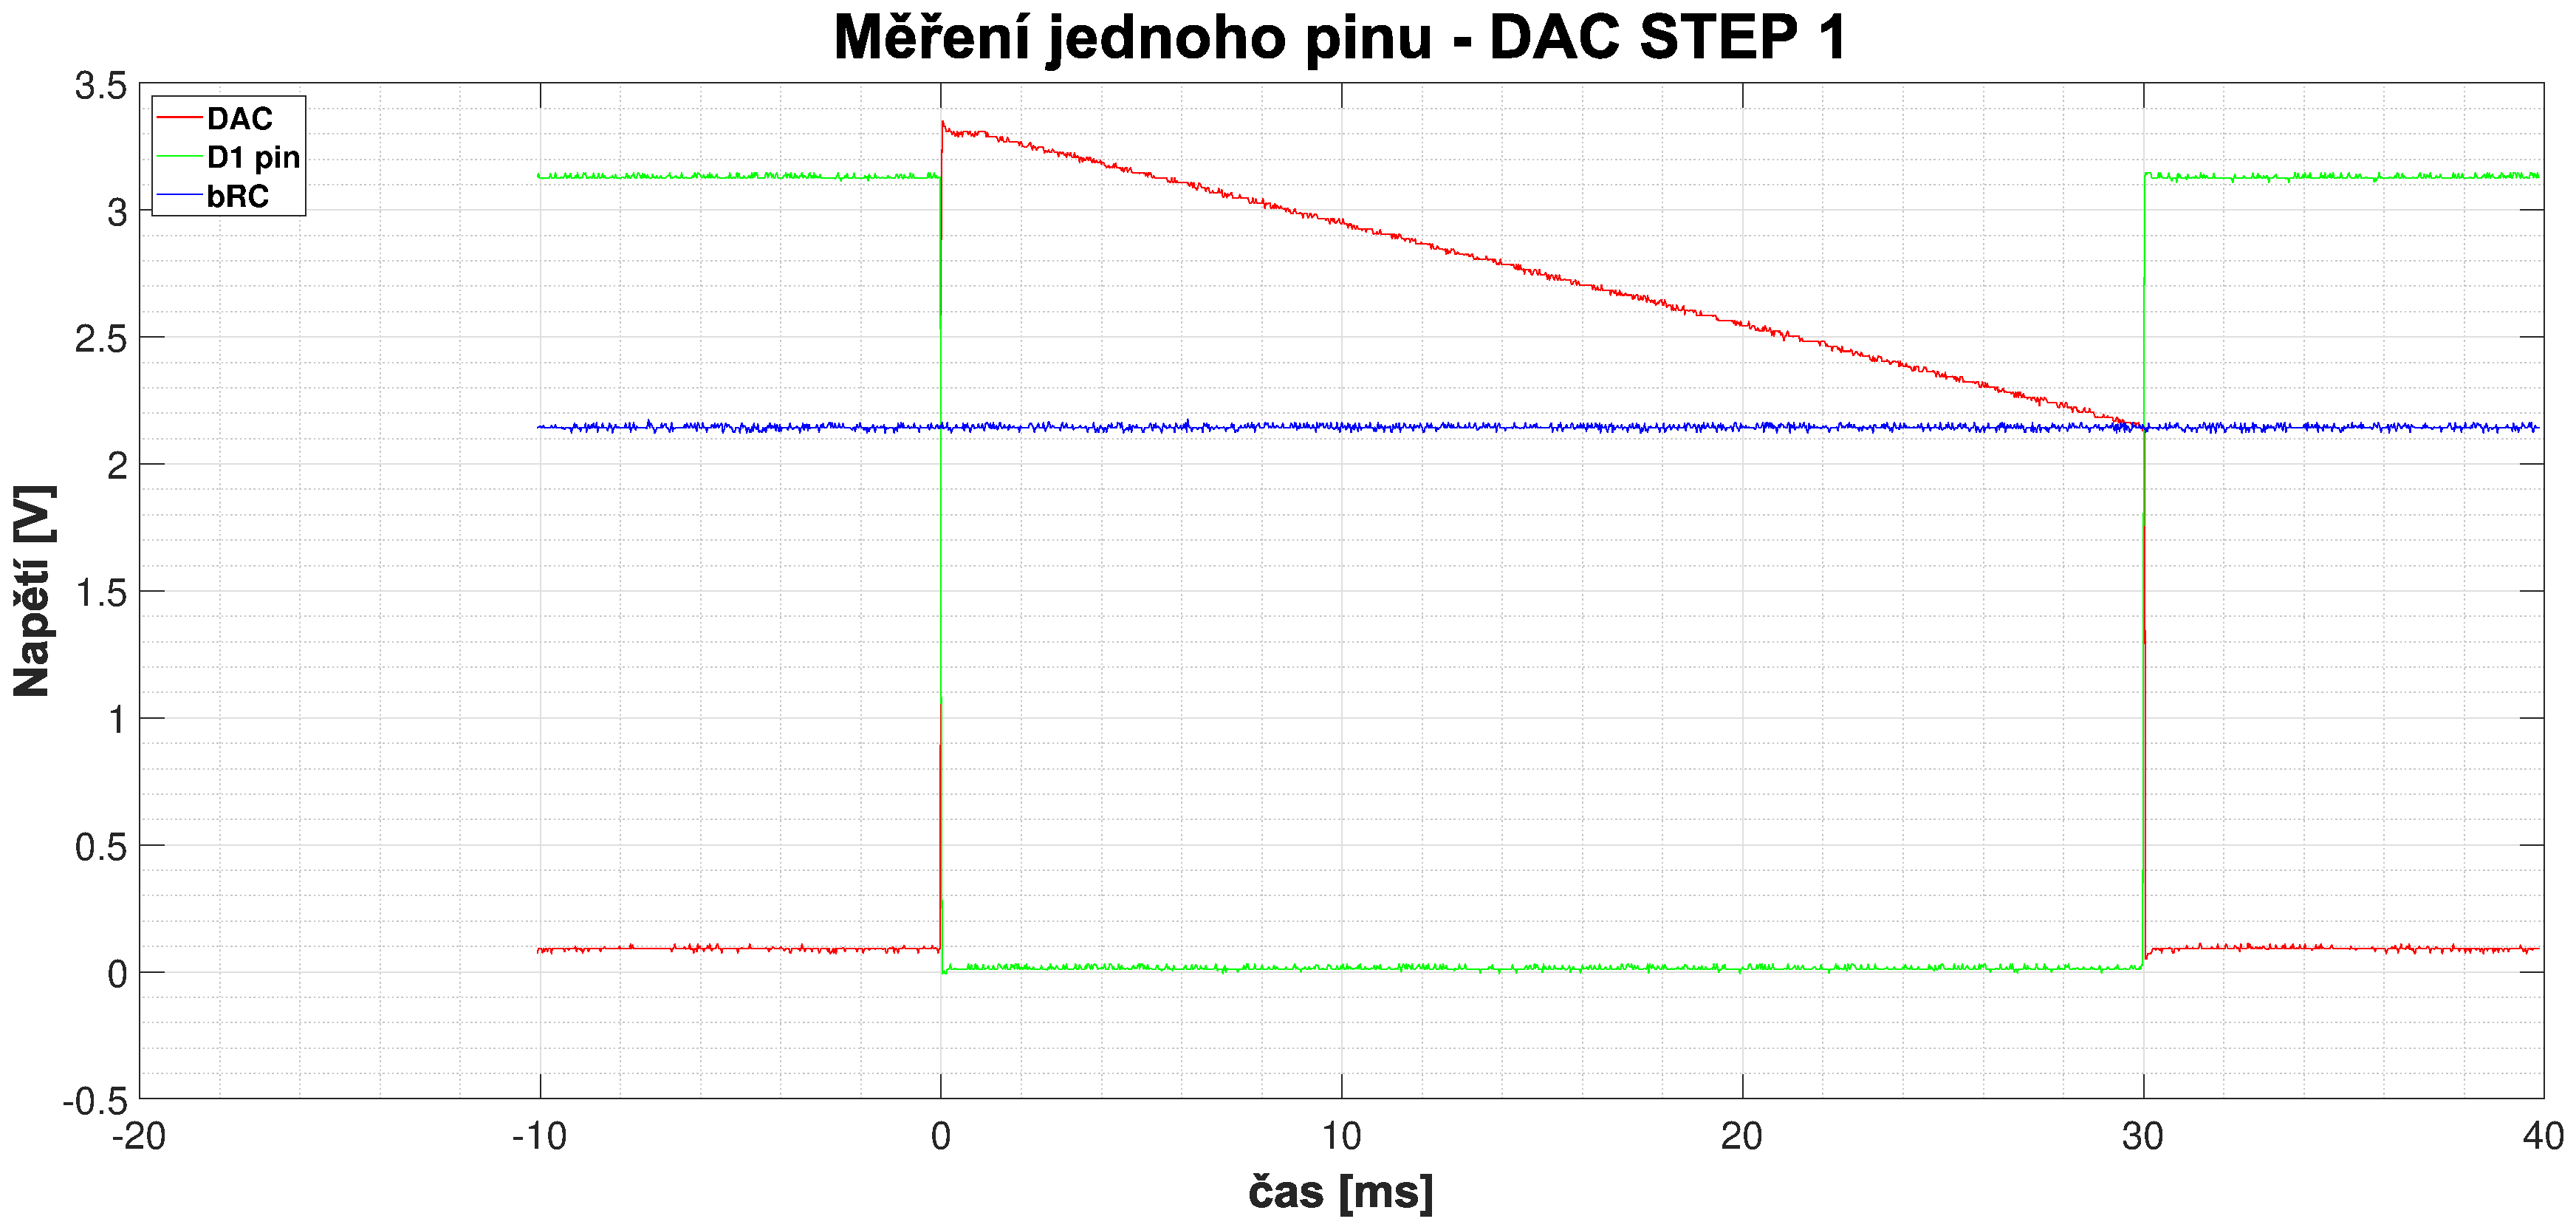
\includegraphics[width = \textwidth]{obrazky/matlab_generated/pin_step1.eps}
	\end{figure}
\end{frame}

\begin{frame} 
	% nadpis snímku
	\frametitle{Koncepce testeru}
	\vspace*{0.5cm}
	\begin{figure}[ht!]
		\centering
		%\includegraphics[width = \textwidth]{obrazky/system_connection.png}
		\includegraphics[width = \textwidth]{obrazky/system_karet_obh.png}
	\end{figure}
\end{frame}


\begin{frame} 
	% nadpis snímku
	\frametitle{Foto propojení měřící a ovládací karty}
	\begin{figure}[ht!]
		\centering
		%\includegraphics[width = \textwidth]{obrazky/system_connection.png}
		\includegraphics[height = 0.7\textwidth, angle = 90]{obrazky/foto_obh.jpg}
	\end{figure}
\end{frame}

\begin{frame} 
	% nadpis snímku
	\frametitle{Měřící karta 1/2}
	\vspace*{0.5cm}
	\begin{figure}[ht!]
		\centering
		%\includegraphics[width = \textwidth]{obrazky/system_connection.png}
		\includegraphics[width = \textwidth]{obrazky/karta_system_diagram.png}
	\end{figure}
\end{frame}

\begin{frame} 
	% nadpis snímku
	\frametitle{Měřící karta  2/2}
	\vspace*{1cm}
	\begin{figure}[ht!]
		\centering
		%\includegraphics[width = \textwidth]{obrazky/system_connection.png}
		\includegraphics[width = \textwidth]{obrazky/all_layers_no_poly.png}
	\end{figure}
\end{frame}

\begin{frame} 
	% nadpis snímku
	\frametitle{Ovládací karta 1/2}

	\begin{figure}[ht!]
		\centering
		%\includegraphics[width = \textwidth]{obrazky/system_connection.png}
		\includegraphics[height = 0.8\textheight]{obrazky/ovladaci_karta_diag.png}
	\end{figure}
\end{frame}

\begin{frame} 
	% nadpis snímku
	\frametitle{Ovládací karta 2/2}

	\begin{figure}[ht!]
		\centering
		%\includegraphics[width = \textwidth]{obrazky/system_connection.png}
		\includegraphics[height = 0.8\textheight]{obrazky/all_layers_no_poly_control.png}
	\end{figure}
\end{frame}

\begin{frame} 
	% nadpis snímku
	\frametitle{Dosažená přesnost měření 1/3}

	\begin{figure}[ht!]
		\centering
		%\includegraphics[width = \textwidth]{obrazky/system_connection.png}
		\includegraphics[width = \textwidth]{obrazky/10hourTestScheme.png}
	\end{figure}
\end{frame}

\begin{frame} 
	% nadpis snímku
	\frametitle{Dosažená přesnost měření 2/3}

	\begin{figure}[ht!]
		\centering
		%\includegraphics[width = \textwidth]{obrazky/system_connection.png}
		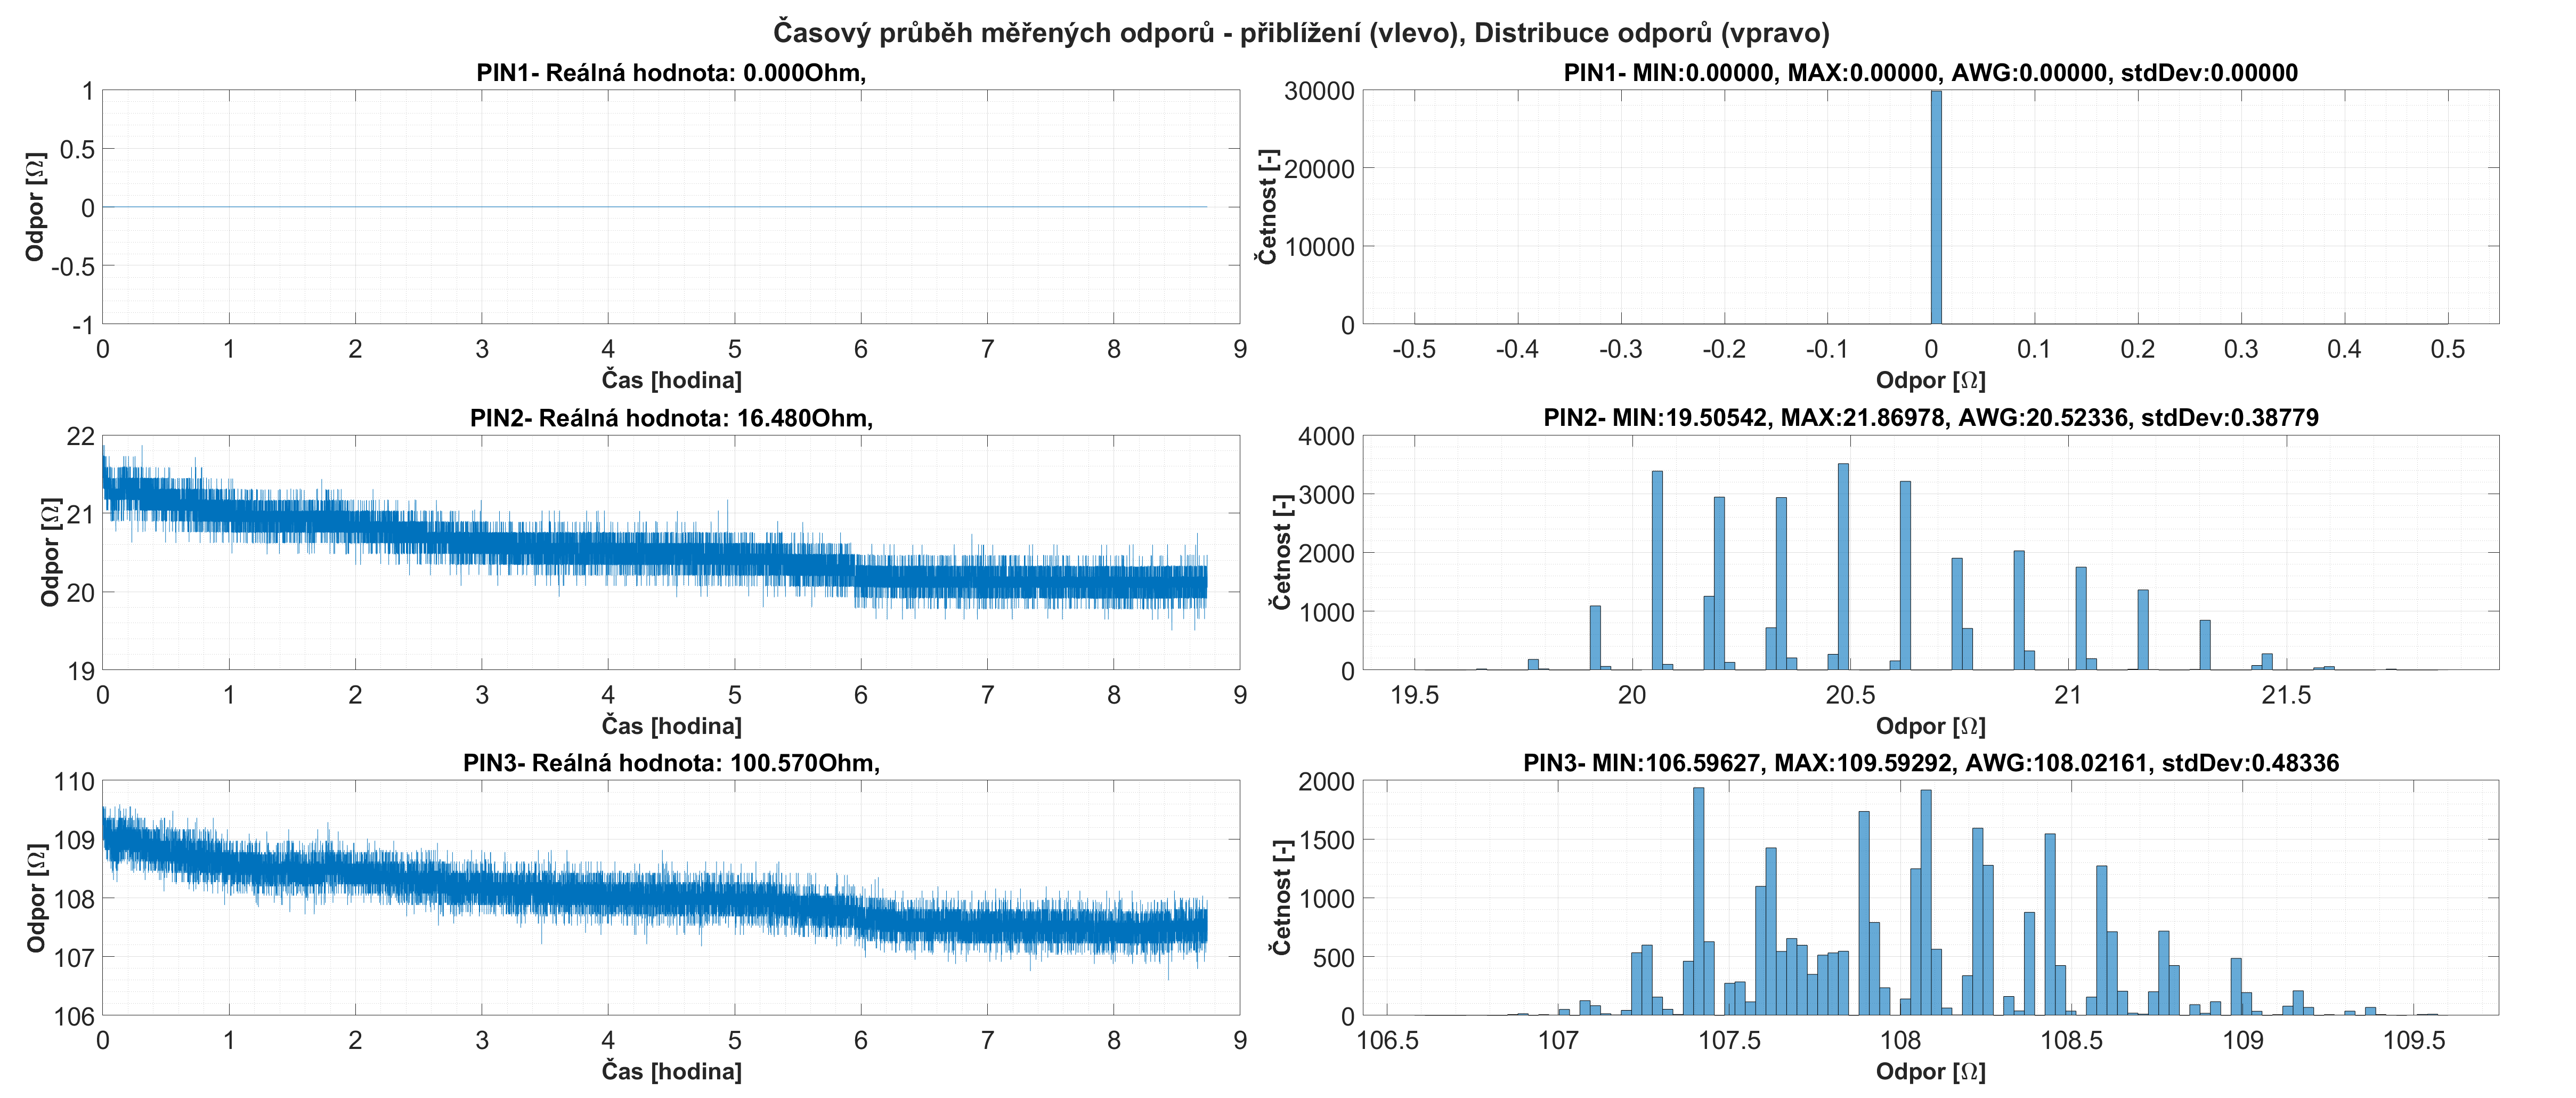
\includegraphics[width = \textwidth]{obrazky/matlab_generated/VOLTAGE_TESTER/dlouhodoba_stabilita_resistor_part1_obhj.eps}
	\end{figure}
\end{frame}

\begin{frame} 
	% nadpis snímku
	\frametitle{Dosažená přesnost a rychlost měření 3/3}
	\vspace*{0.7cm}
	\begin{table}[ht!]
	\centering
		\resizebox{0.7\textwidth}{!}{%
		\begin{tabular}{|l|l|l|l|l|l|}
		\hline
		-        & \textbf{PIN2} & \textbf{PIN3} & \textbf{PIN4} & \textbf{PIN5} & \textbf{PIN6} \\ \hline
		\textbf{ref odpor {[}$\Omega${]}}  & 16.5     & 100.57     & 180.77     & 996.75      & 4673.19 \\ \hline
		\textbf{abs chyba {[}$\Omega${]}}  & 0.11     & 0.62      & 2.15     & 17.61      & 34.42     \\ \hline
		\textbf{rel chyba {[}\%{]}} & 0.647      & 0.616      & 1.189      & 1.767      & 0.737      \\ \hline
		\end{tabular}%
		}
		\caption{Chyby měření odporů vůči pinu č. 1}
		\label{tab:chyby mereni calibrated}
	\end{table}

	\begin{itemize}
		\item Čas měření v PASS/FAIL režimu je závislý převážně na rychlosti zpracování PC aplikace. Obvyklá odezva aplikace je do 50ms.
	\end{itemize}
\end{frame}





\begin{frame} 
	% nadpis snímku
	\frametitle{PC aplikace 1/2}

	\begin{figure}[ht!]
		\centering
		%\includegraphics[width = \textwidth]{obrazky/system_connection.png}
		\includegraphics[width = 1\textwidth]{obrazky/PC_APP_dataViewer.png}
	\end{figure}
\end{frame}

\begin{frame} 
	% nadpis snímku
	\frametitle{PC aplikace 2/2}

	\begin{figure}[ht!]
		\centering
		%\includegraphics[width = \textwidth]{obrazky/system_connection.png}
		\includegraphics[width = 1\textwidth]{obrazky/PC_APP_CONTROL_PANEL.png}
	\end{figure}
\end{frame}

%%%%%%%%%%%%%
\begin{frame} 
	\frametitle{Pokračování DP}
	\vspace*{0.5cm}
	\begin{itemize}
		\item Finalizace mechanické konstrukce testeru
		\item Ethernet bootloader
		\item Odladění v "ostrém"\ provozu
		\item Ověření dlouhodobé spolehlivosti
		\item Vylepšení CSS stylů PC aplikace
		\item Rozšíření PC aplikace
	\end{itemize}
\end{frame}


% podekovani
\begin{frame}[c] 
% bez nadpisu snímku
	\frametitle{\mbox{ }}
	\begin{center}
		{\Huge Děkuji za pozornost!}
	\end{center}
\end{frame}


% otázky oponenta
\frame{
\frametitle{Otázky oponenta}
\begin{itemize}
	\item \textbf{Uveďte, na kterých částech zařízení jste pracoval sám a zda jste u některých bloků využil spolupráci s kolegy z firmy.}\\
	\item \textbf{Jak často se bude provádět kalibrace zařízení, jednou po sestavení převodníku nebo periodicky?}\\
	\item \textbf{Proč nebyla pro měření použita metoda postupné aproximace (půlení intervalu)? Bylo by takto možné urychlit měření přesného odporu?}\\
\end{itemize}
}

\frame{
\frametitle{Otázky oponenta - Spolupráce kolegů}
\vspace*{1.5cm}
\begin{center}
	{\Huge Uveďte, na kterých částech zařízení jste pracoval sám a zda jste u některých bloků využil spolupráci s kolegy z firmy.}
\end{center}
}

\begin{frame} 
	% nadpis snímku
	\frametitle{Spolupráce kolegů}
	\begin{figure}[ht!]
		\centering
		%\includegraphics[width = \textwidth]{obrazky/system_connection.png}
		\includegraphics[height = 0.8\textheight]{obrazky/assembly_3D_model.png}
	\end{figure}
\end{frame}


\frame{
\frametitle{Otázky oponenta - Kalibrace}
\vspace*{1.5cm}
\begin{center}
	{\Huge Jak často se bude provádět kalibrace zařízení, jednou po sestavení převodníku nebo periodicky?}
\end{center}
}

\begin{frame} 
	% nadpis snímku
	\frametitle{Otázky oponenta - Kalibrace}
	\vspace*{1.2cm}
	\begin{figure}[ht!]
		\centering
		%\includegraphics[width = \textwidth]{obrazky/system_connection.png}
		\includegraphics[width = \textwidth]{obrazky/kalibrace_obh.png}
	\end{figure}
\end{frame}

\frame{
\frametitle{Otázky oponenta - metoda postupné aproximace}
\vspace*{1.5cm}
\begin{center}
	{\Huge Proč nebyla pro měření použita metoda postupné aproximace (půlení intervalu)? Bylo by takto možné urychlit měření přesného odporu?}
\end{center}
}

\begin{frame} 
	% nadpis snímku
	\frametitle{Otázky oponenta - metoda postupné aproximace 1/4}
	\vspace*{0.5cm}
	\begin{figure}[ht!]
		\centering
		%\includegraphics[width = \textwidth]{obrazky/system_connection.png}
		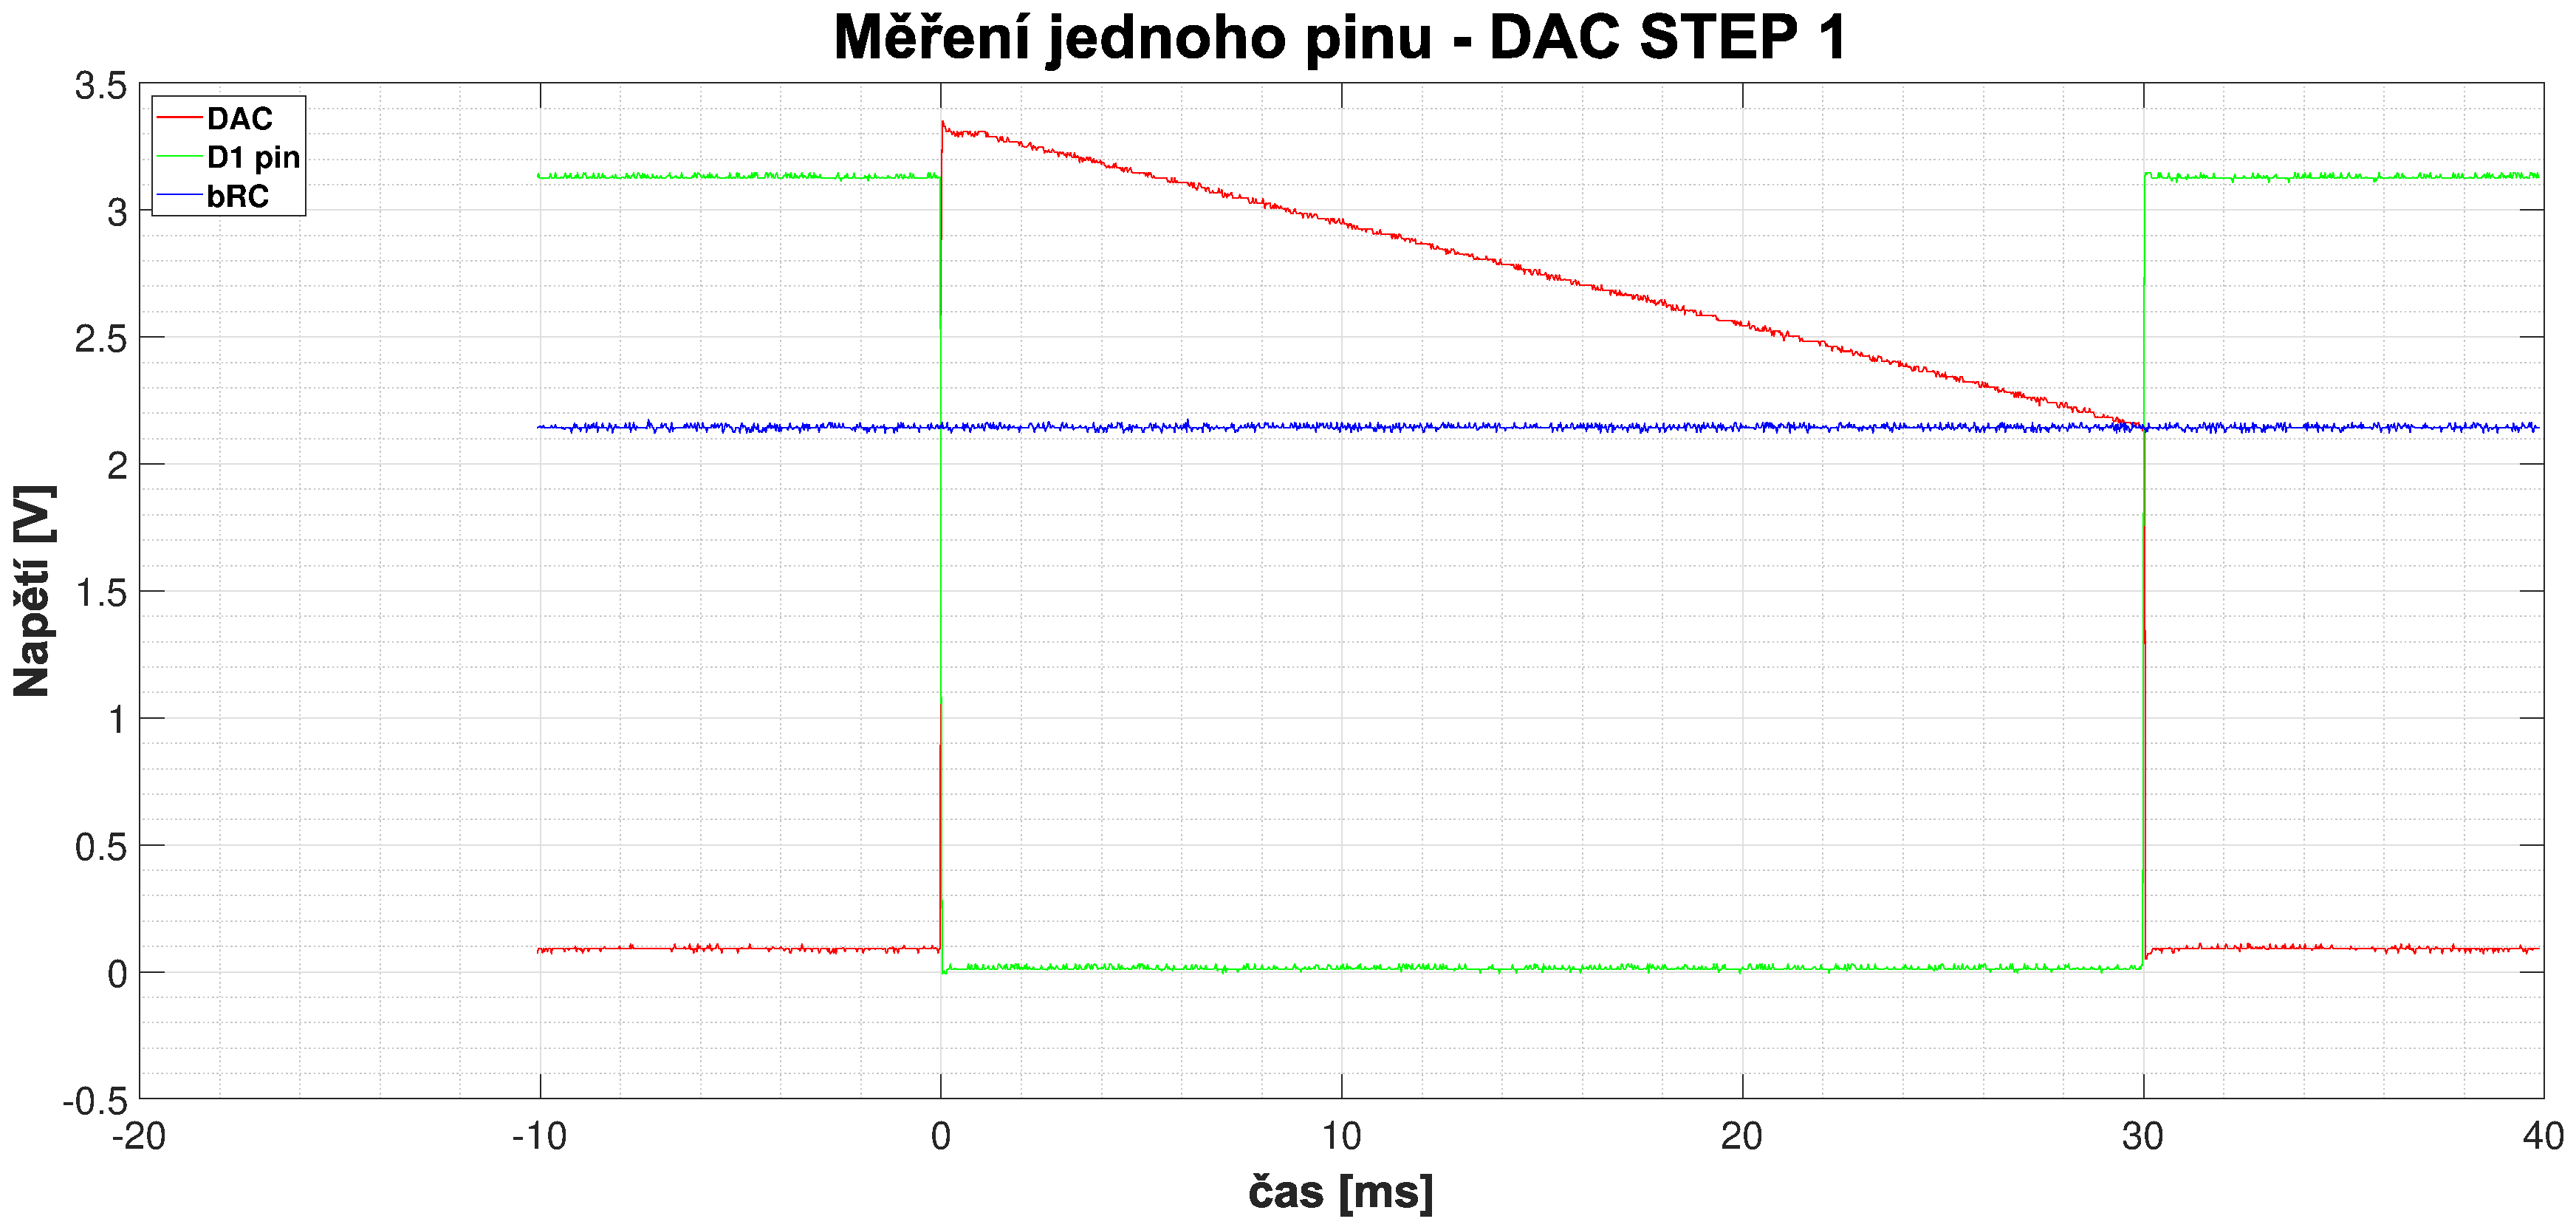
\includegraphics[width = \textwidth]{obrazky/matlab_generated/pin_step1.eps}
	\end{figure}
\end{frame}

\begin{frame} 
	% nadpis snímku
	\frametitle{Otázky oponenta - metoda postupné aproximace 2/4}
	\vspace*{0.5cm}
	\begin{figure}[ht!]
		\centering
		%\includegraphics[width = \textwidth]{obrazky/system_connection.png}
		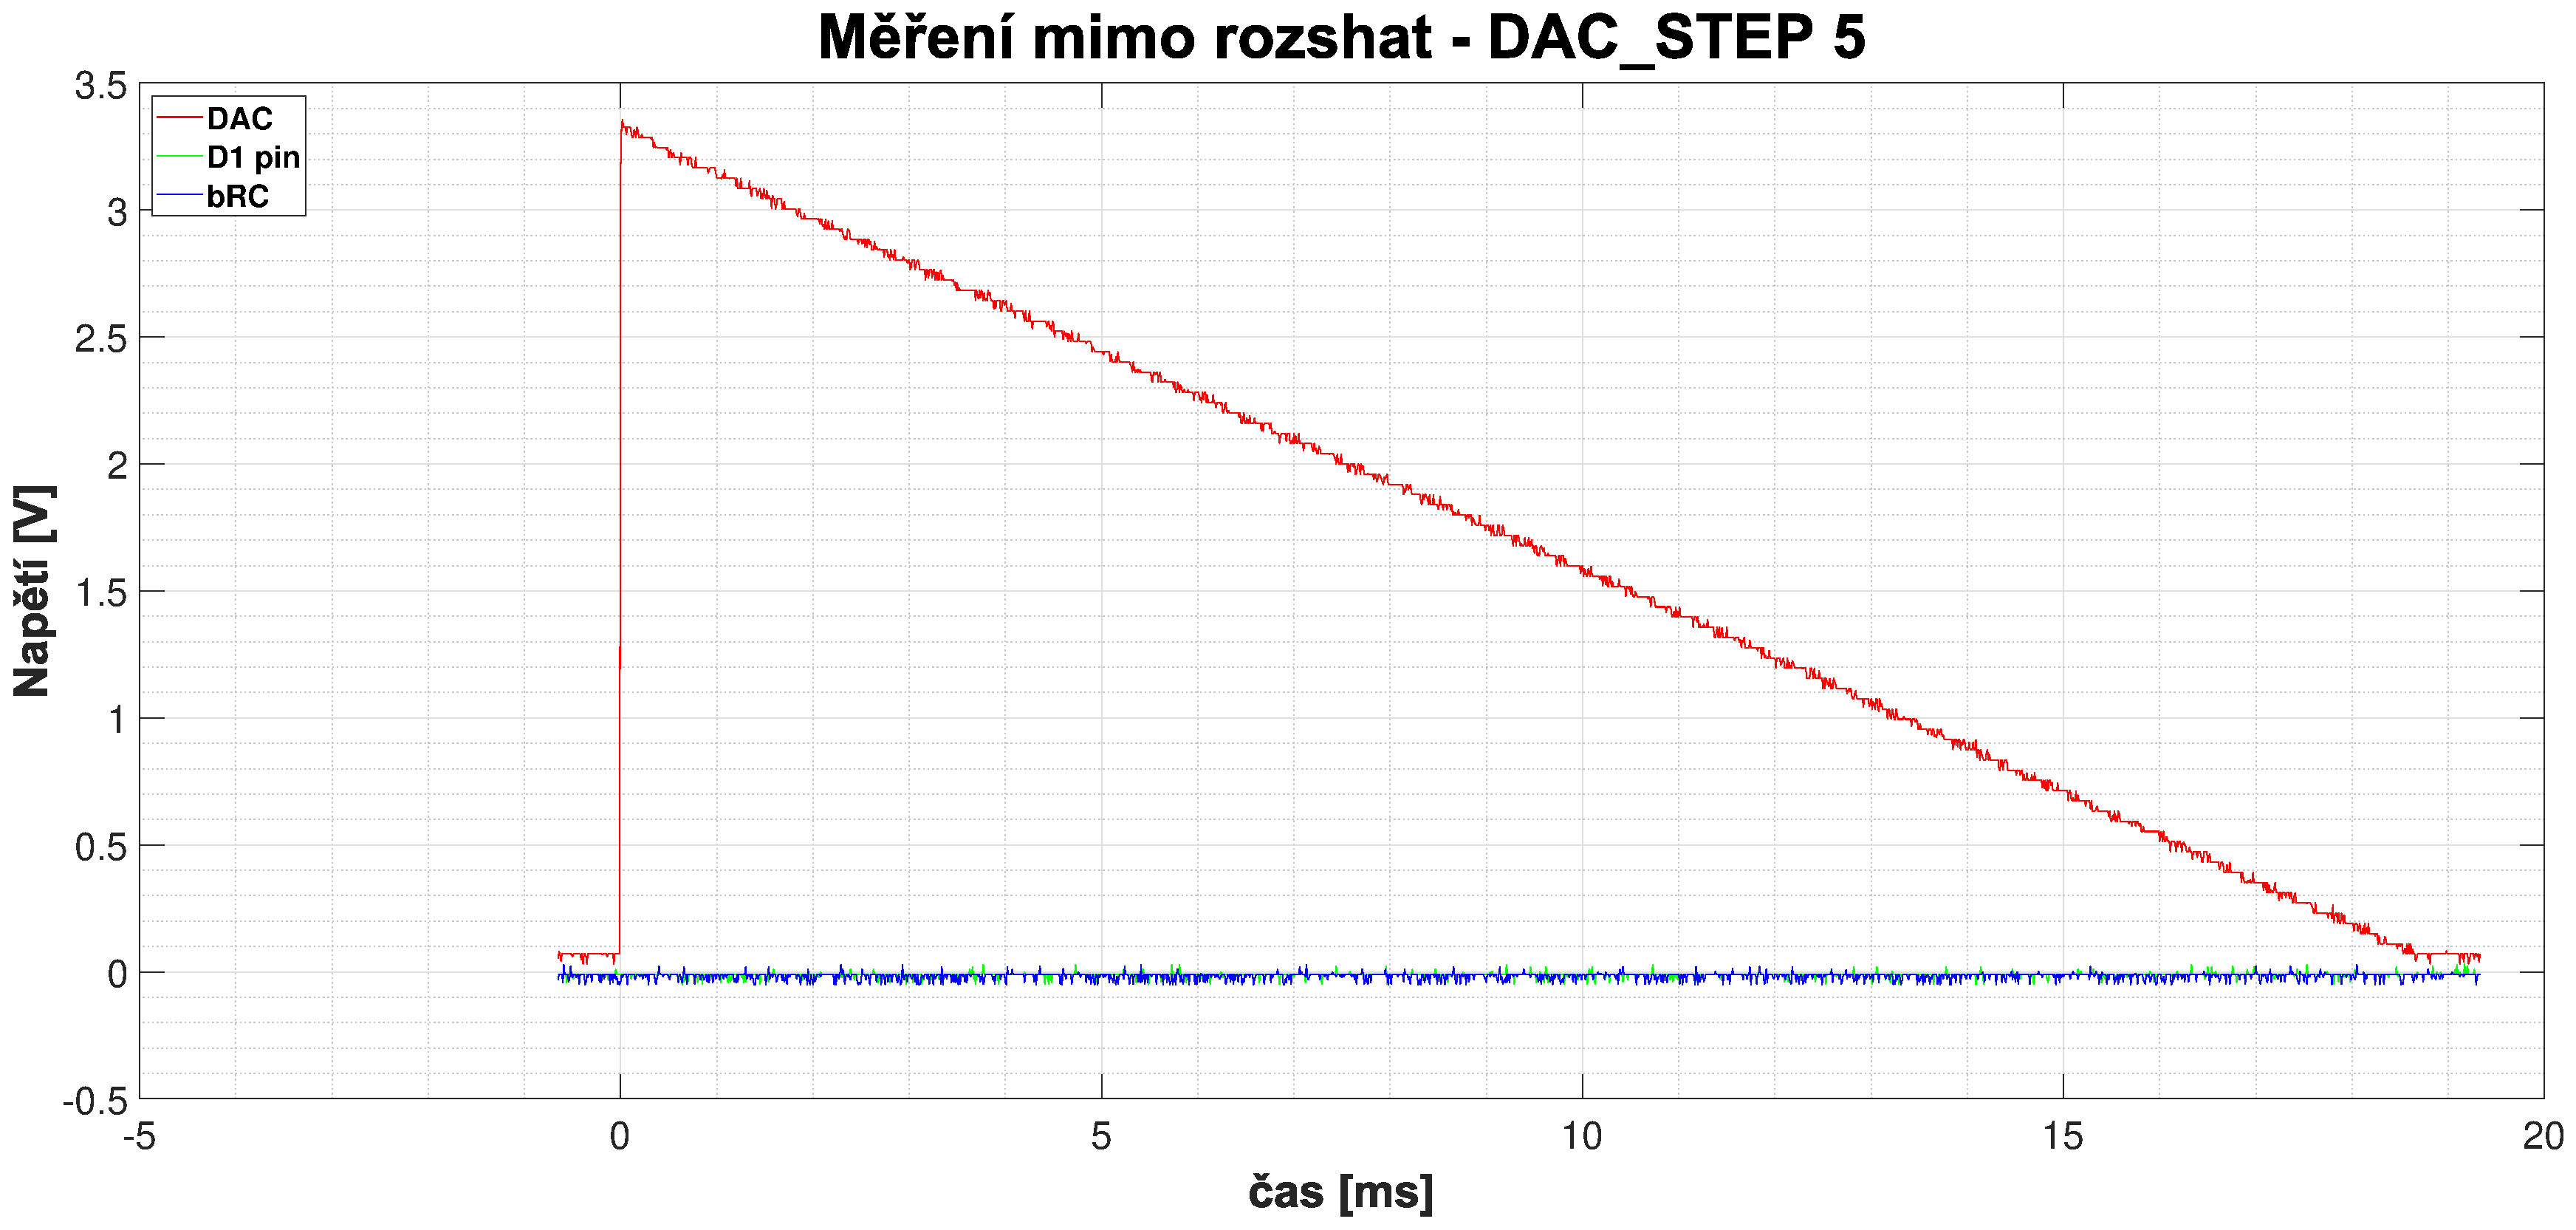
\includegraphics[width = \textwidth]{obrazky/matlab_generated/pin_out_of_range.eps}
	\end{figure}
\end{frame}


\begin{frame} 
	% nadpis snímku
	\frametitle{Otázky oponenta - metoda postupné aproximace 3/4}
	\vspace*{0.5cm}
	\begin{figure}[ht!]
		\centering
		%\includegraphics[width = \textwidth]{obrazky/system_connection.png}
		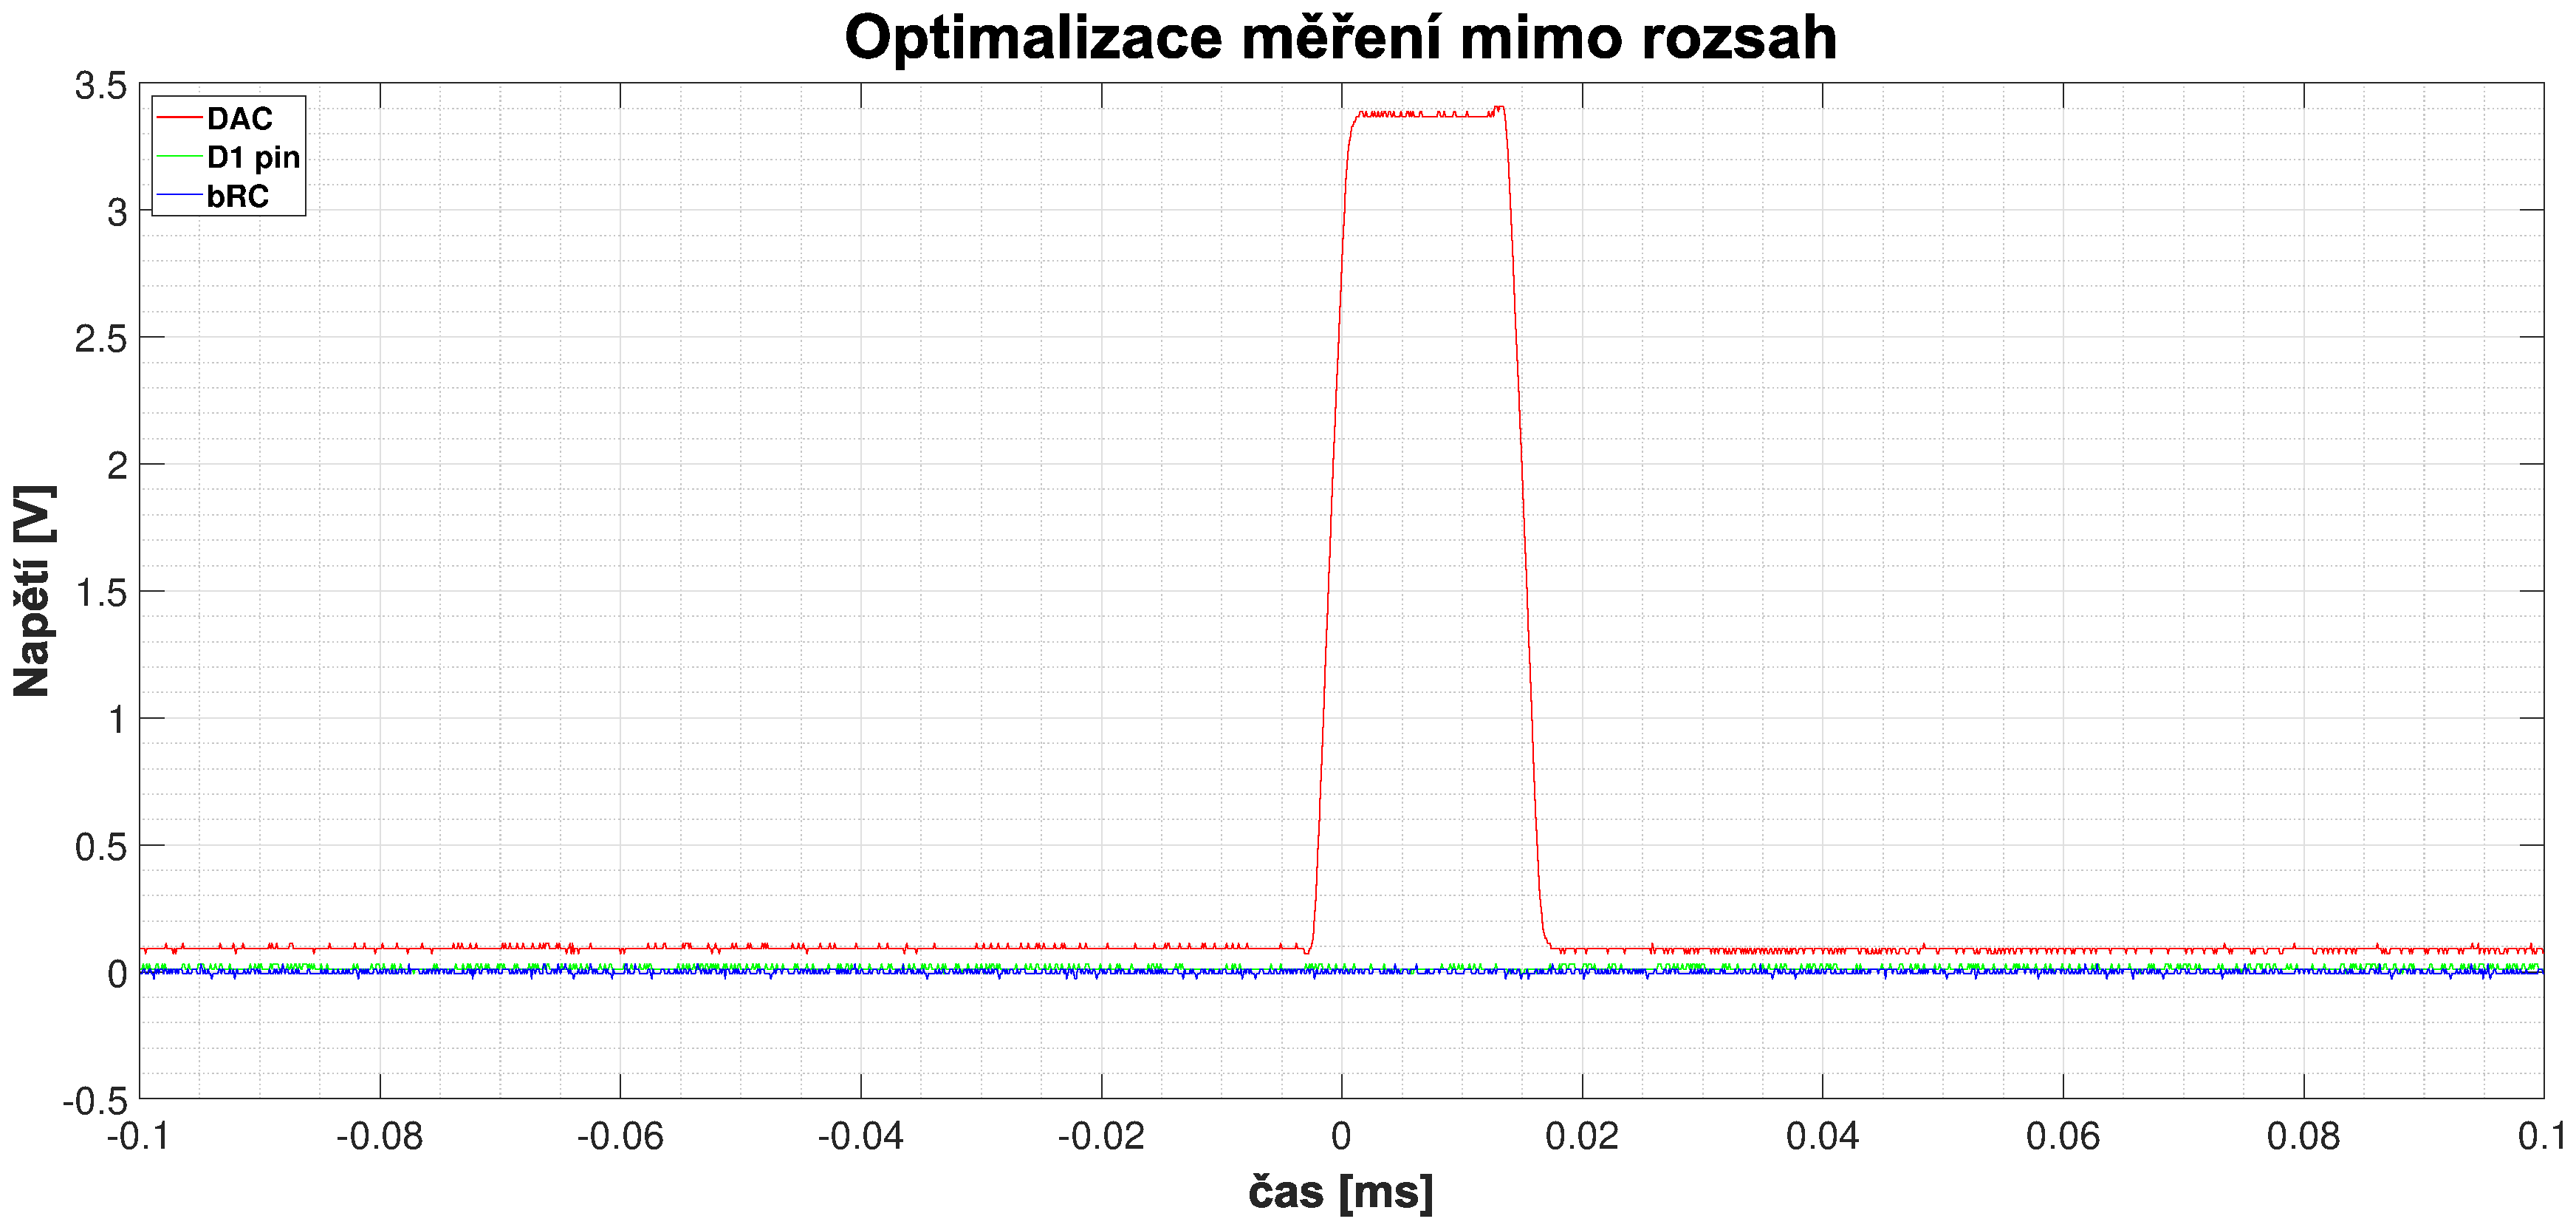
\includegraphics[width = \textwidth]{obrazky/matlab_generated/pin_out_of_range_opt.eps}
	\end{figure}
\end{frame}


\begin{frame} 
	% nadpis snímku
	\frametitle{Otázky oponenta - metoda postupné aproximace 4/4}
	\vspace*{0.5cm}
	\begin{figure}[ht!]
		\centering
		%\includegraphics[width = \textwidth]{obrazky/system_connection.png}
		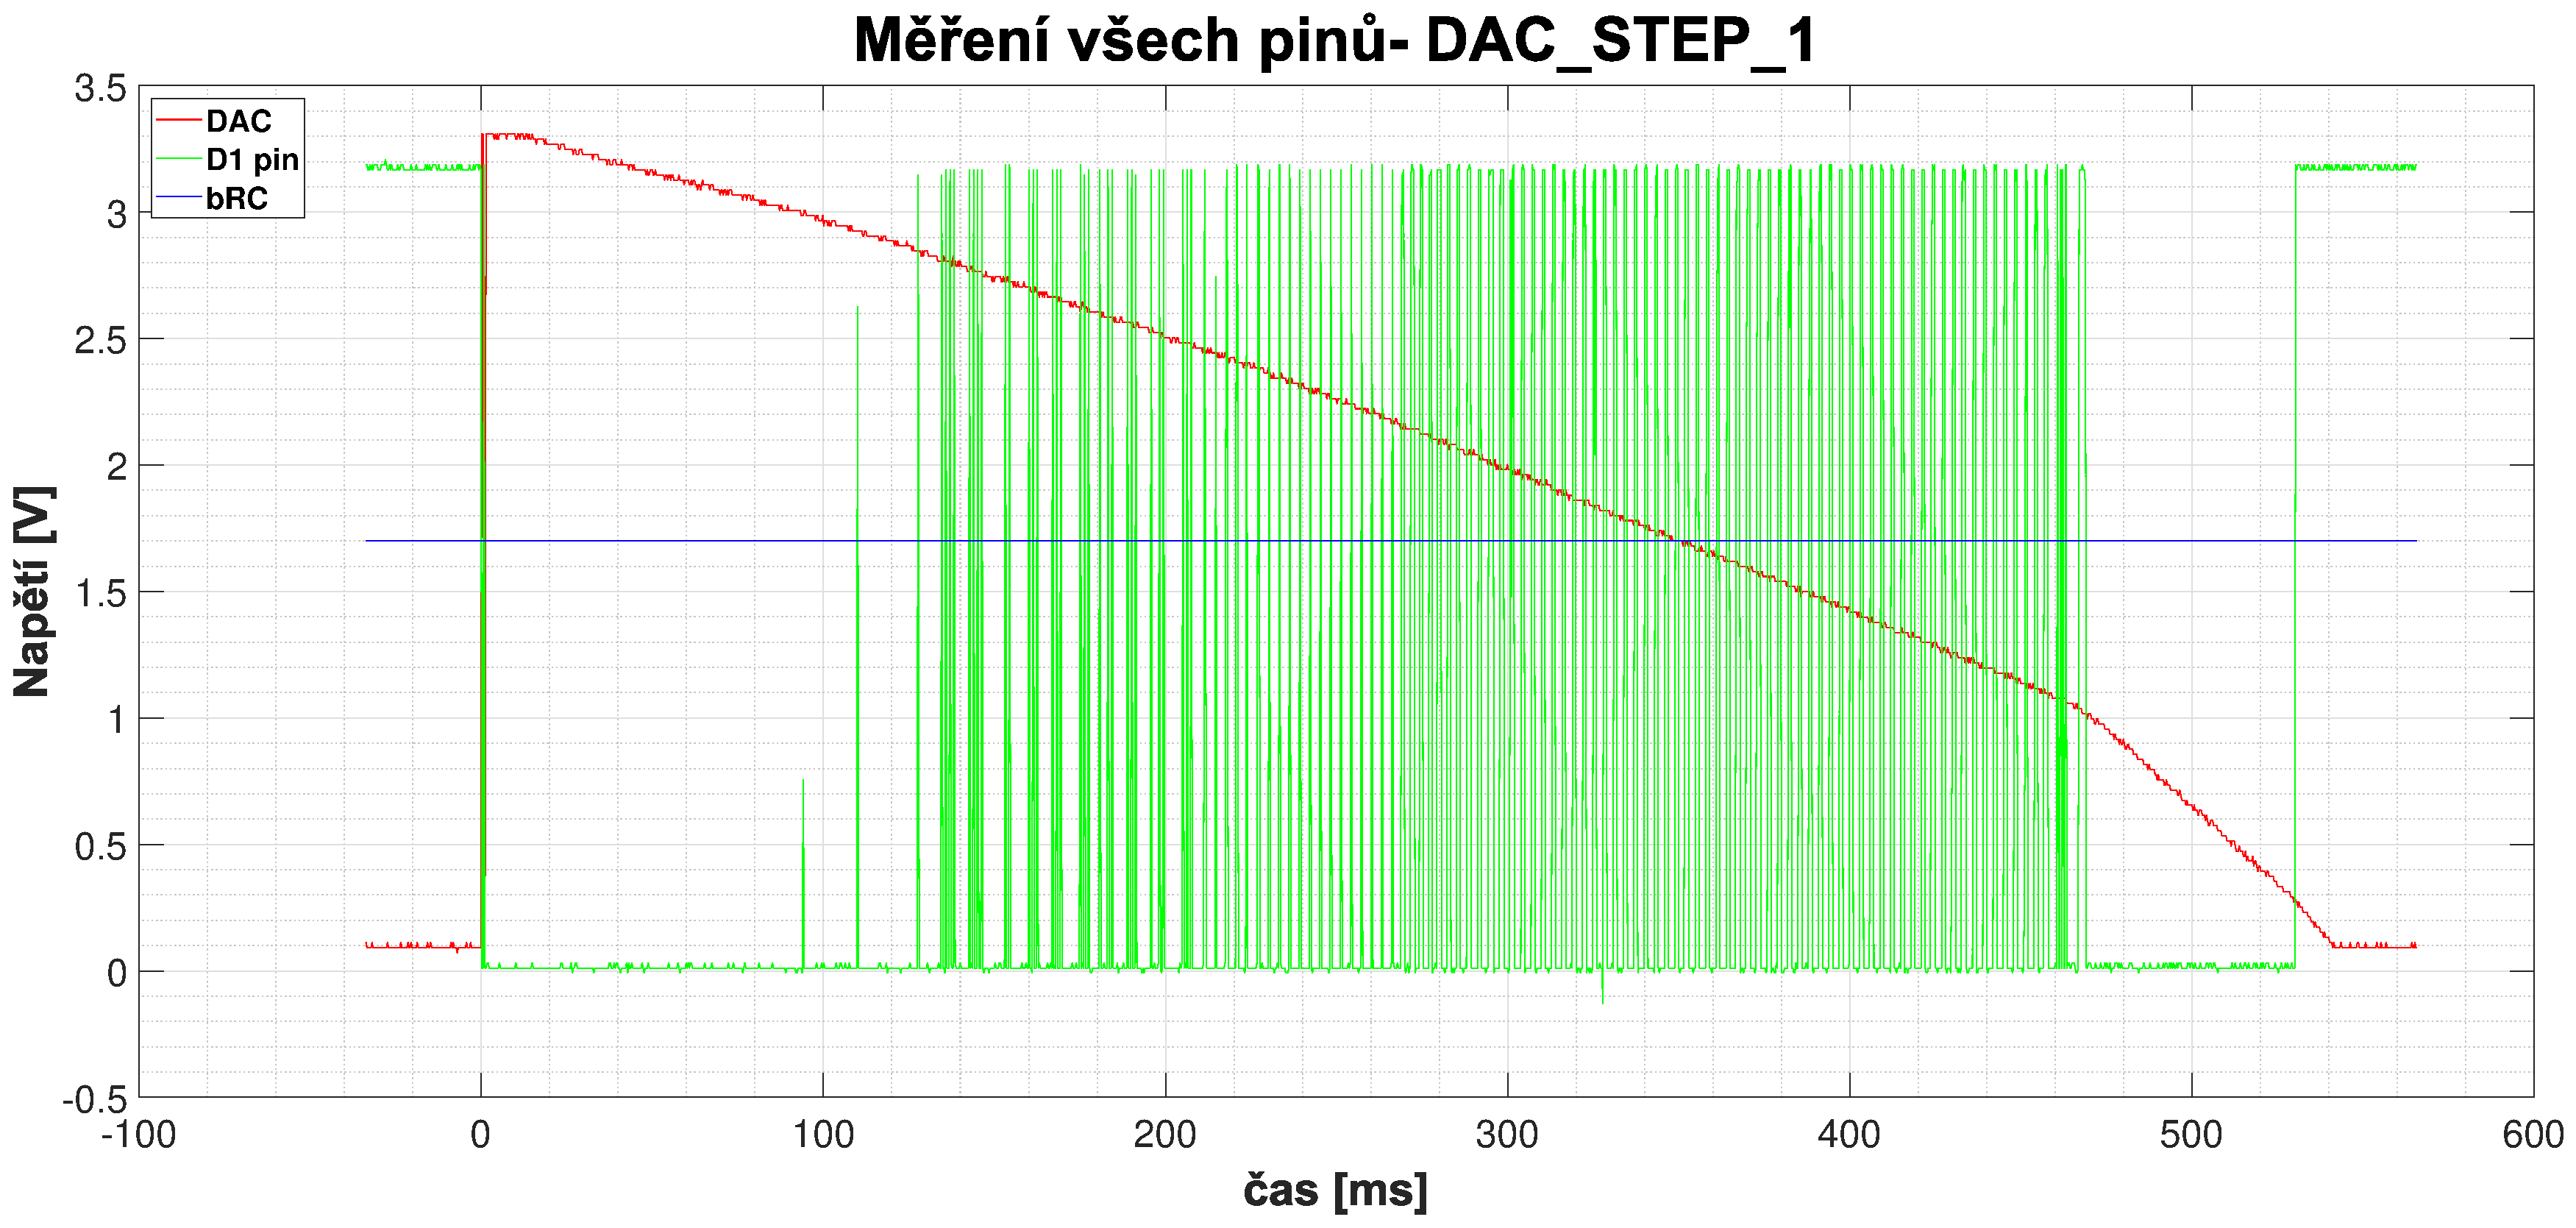
\includegraphics[width = \textwidth]{obrazky/matlab_generated/all_pins.eps}
	\end{figure}
\end{frame}


\end{document}
